\documentclass[fontsize=12pt,toc=bibliography, notitlepage]{scrreprt}

\usepackage[english]{babel}
\usepackage{ucs}
\usepackage[utf8x]{inputenc}
\usepackage[bookmarksopen=true,
			bookmarks=true,
			plainpages=false,
        	pdfpagelabels=true,
			colorlinks=true,
			linkcolor=black,
			citecolor=black,
        	filecolor=black,
        	urlcolor=blue]{hyperref}
\usepackage{graphicx}
\usepackage{float}
\usepackage{listings}
\usepackage{color}
\usepackage{tikz}

\title{Heart Rate Monitor}
\subtitle{Ubiquitous Computing Mini Project}
\author{Fabian Meyer \and Jens Gansloser}
\date{\today \\ HTWG Konstanz}

\lstdefinestyle{MyCStyle}{
  belowcaptionskip=1\baselineskip,
  breaklines=true,
  frame=single,
  captionpos=b,
  numbers=left,
  xleftmargin=\parindent,
  language=C,
  showstringspaces=false,
  basicstyle=\footnotesize\ttfamily,
  keywordstyle=\bfseries\color{green!40!black},
  commentstyle=\itshape\color{purple!40!black},
  identifierstyle=\color{blue},
  stringstyle=\color{orange}
}
\lstset{escapechar=@,style=MyCStyle}

\begin{document}

\maketitle
\begin{abstract}
The aim of this project is to build a heart rate monitor. There are already a lot of devices commercially available which measure the heart rate. However, the internal functionality of these devices is not exposed to the user, so there cannot be made any statements about their precision and the quality of the results. Additionally, most devices need to be worn on the users chest or the user must place his finger on it.
\end{abstract}
\clearpage

\tableofcontents

\chapter{Principle of Operation}
\label{chap:principle-of-operation}

\section{Pulse Rate}
\label{sec:pulse-rate}
An alternative method to measure the heart rate is the photoplethysmogram (PPG) technique. This method measures the change of the blood volume through the absorption or reflection of light.\\
A light emitting diode (LED) shines through a thin amount of tissue (e.g. fingertip, earlobe). The wavelength of the light should be in near infrared area. On the other side a photodiode registers the intensity of light that traversed the tissue. Since blood changes its color with its grade of oxygenation, more or less light of the LED gets absorbed by it. If the heart pushes blood through the vessels, more oxygenated blood lays between the LED and photodiode. As a result the registered intensity of light changes continously with the pulse. By measuring the time between two intensity peaks the current pulse can be estimated.\\
The setting for the pulse rate monitor is displayed in figure \ref{fig:pulse-rate-monitor-setting}.

\begin{figure}[H]
	\centering
	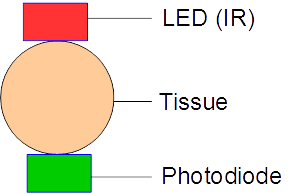
\includegraphics[width=200px]{images/pulse-rate-aufbau.png}
	\caption{Pulse Rate Monitor Setting}
	\label{fig:pulse-rate-monitor-setting}
\end{figure}

\section{Oxygen Saturation}
\label{sec:oxygen-saturation}
The oxygen saturation of the blood can be measured by using 2 light emitting diodes . One LED emitting light with a wavelength of 660nm (red light) and the other one emitting light with a wavelength of 940nm (infrared light). The absorption of light by blood changes corresponding to its oxygen saturation. Oxygenated blood absorbs more infrared light and less red light. With de-oxygenated blood it is the other way around \cite{bib:pulse-oximetry}. The LEDs blink alternating and a photodiode is used to measure the light intensity after the light traversed the tissue. These measurements in combination with the Lambert-Beer-Law are used to calculate the oxygen saturation.

\chapter{Environment}
\label{chap:environment}

\begin{figure}[H]
	\centering
	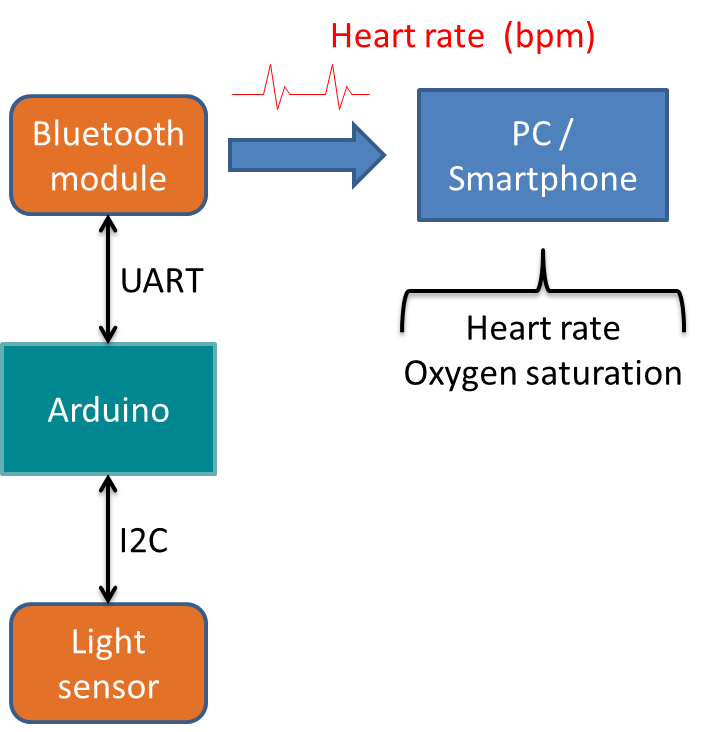
\includegraphics[width=200px]{images/general_dataFlow.png}
	\caption{Data Flow}
	\label{fig:data-flow}
\end{figure}

\section{Light Intensity Sensor}
\label{sec:light-intensity-sensor}

\subsection{Hardware}
\label{subsec:light-intensity-sensor-hardware}
To measure light, the 16bit TSL2561 Luminosity Sensor breakout board from Adafruit is used.
It provides the TSL2561 Light-To-Digital Converter which is able to sense full spectrum and IR light with a very high sensitivity (see graphic below). The sensor contains of a broadband photodiode (visible and infrared) and a infrared photodiode. Two ADCs convert the analog data to digital data, that can be read via the I$^{2}$C bus. The light sensor can be configured with different gain, which changes the sensitivity to light. This is needed if the sensor is used in areas with bright light or low light. A second option to configure is the integration time (13ms, 101ms, 402ms). This configures the resolution of the device, so that the sensor has more time to take samples. With a integration time of 402ms, the sensor has the complete 16bit resolution. The output of the sensor can be used to calculate the measured SI-Unit lux, which indicates the illuminance.\cite{bib:tsl-sensor}\\
Figure \ref{fig:tsl-2561-spectrum} shows the light spectrum of the two photodiodes on the board.

\begin{figure}[H]
	\centering
	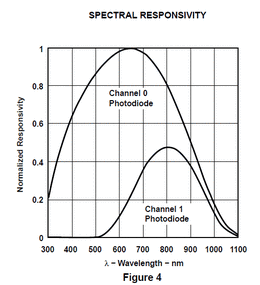
\includegraphics[width=200px]{images/light_tsl2561spectrum.png}
	\caption{TSL-2561 Spectrum}
	\label{fig:tsl-2561-spectrum}
\end{figure}

\subsection{Software}
\label{subsec:light-intensity-sensor-software}
To get data from the light sensor, the Adafruit TSL2561 and Adafruit Unified Sensor Driver library are used. These libraries do the I$^{2}$C communication and the digital to lux calculation. Also they provide functions to set the gain and integration time options. \cite{bib:tsl-library} \cite{bib:sensor-library}

\begin{lstlisting}
tsl.enableAutoRange(true);
tsl.setIntegrationTime(TSL2561_INTEGRATIONTIME_13MS);

uint16_t broadband, ir;
tsl.getLuminosity(&broadband, &ir);
\end{lstlisting}

Line 1 sets the gain value to auto range. That means it adapts automatically to the sensors environment. On line 2 the integration time is set to 13ms (low resolution, fast processing). Line 5 querys for the luminosity values of the broadband and ir photodiode.

\section{Microcontroller}
\label{sec:microcontroller}
The data of the sensor is further computed by an Arduino Board from Adafruit \cite{bib:arduino-board}. The board receives the data of the sensor via I$^{2}$C bus system and interprets it according to the case if a pulse happened or not. Using the time difference between two pulses the microcontroller is able to estimate the current pulse.
The board uses an ATmega328 CPU with 16MHz clockrate.

\section{Communication Device}
\label{sec:communication-device}

\subsection{Hardware}
\label{subsec:bluetooth-adapter-hardware}
The Bluefruit EZ-Link is a serial link bluetooth module. That means, the Arduino can communicate via UART with the bluetooth module, which handles the wireless transmission to the computer. On the computer side, the module (if it was paired successfully) is recognized as an serial port (COM). See also \cite{bib:bluetooth-adapter}.

\chapter{The Project}
\label{chap:the-project}

\section{Tests}
\label{sec:tests}
For first tests, a GUI-Application running on a pc is used. This application receives the broadband and ir values from the sensor and displays it graphically.
The next step is to analyse the received data and try different sensor settings.

\begin{figure}[H]
	\centering
	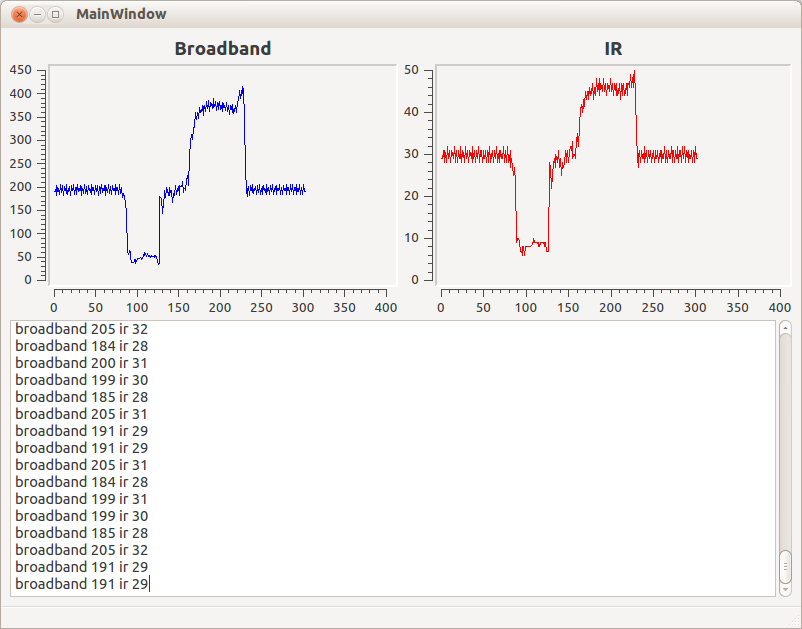
\includegraphics[width=350px]{images/hrm.png}
	\caption{Heartrate Monitor}
	\label{fig:heartrate-monitor}
\end{figure}

\section{Wiring}
\label{sec:wiring}

\section{Bluetooth Protocol}
\label{sec:bluetooth-protocol}

\begin{thebibliography}{999}
	\bibitem{bib:pulse-oximetry} Pulse Oximetry, Dr. Chloe Borton, \url{http://www.patient.co.uk/doctor/pulse-oximetry}, 30.05.2014
	\bibitem{bib:tsl-sensor} TSL2561, \url{https://learn.adafruit.com/tsl2561/overview}, 30.05.2014
	\bibitem{bib:arduino-board} Arduino Board, \url{http://www.adafruit.com/product/50}, 31.05.2014
	\bibitem{bib:bluetooth-adapter} Bluefruit EZ-Link, \url{https://learn.adafruit.com/introducing-bluefruit-ez-link/overview}, 31.05.2014
	\bibitem{bib:tsl-library} TSL 2561 Library, \url{https://github.com/adafruit/Adafruit_TSL2561}, 31.05.2014
	\bibitem{bib:sensor-library} Adafruit Unified Sensor Driver library, \url{https://github.com/adafruit/Adafruit_Sensor}, 31.05.2014
\end{thebibliography}

\cleardoublepage
\addcontentsline{toc}{chapter}{\listfigurename}
\listoffigures

\end{document}